\documentclass[12pt, twoside]{article}
\usepackage[letterpaper, margin=1in, head=30pt, headsep=0.1in]{geometry}
\usepackage[english]{babel}
\usepackage[utf8]{inputenc}
\usepackage{amsmath}
\usepackage{amsfonts}
\usepackage{amssymb}
\usepackage{tikz}
\usepackage{yhmath} %arcs using \wideparen{}
\usetikzlibrary{quotes, angles}

\usepackage{graphicx}
\usepackage{enumitem}
\usepackage{multicol}

%\usepackage{pgfplots}
%\pgfplotsset{width=10cm,compat=1.9}
%\usepgfplotslibrary{statistics}
%\usepackage{pgfplotstable}
%\usepackage{tkz-fct}
%\usepackage{venndiagram}

\usepackage{fancyhdr}
\pagestyle{fancy}
\fancyhf{}
\renewcommand{\headrulewidth}{0pt} % disable the underline of the header
\raggedbottom
\newif\ifmeta
\metatrue %print standards and topics tags

\title{High School Geometry problem sets}
\author{Chris Huson}
\date{April 2021}

%\fancyhead[RE]{\thepage}
%\fancyhead[RO]{\thepage \\ Name: \hspace{3cm}}
%\fancyhead[L]{BECA / Dr. Huson / 10th Grade Geometry\\* 7 June 2019}
%
%\begin{document}
%\subsubsection*{13.7 Homework: Cross sections, distance applications}
%\fancyhead[L]{BECA / Dr. Huson / Geometry 03-Volume+angle-bisectors\\* pset ID: 34}

\begin{document}

\subsubsection*{8.6 Quiz Circle Sectors}
\begin{enumerate}
  \item The shaded sector of the unit circle is \emph{one eighth} of the whole circle, as shown. \\(Circle circumference and area formulas: $C=2\pi r$, $A=\pi r^2$)
  \begin{multicols}{2}
  \raggedcolumns
  \begin{enumerate}[itemsep=1.5cm]
    \item Find $m \angle AOB$ in \emph{degrees}.
    \item Find the length of the arc $\wideparen{AB}$ in terms of $\pi$.
    \item Find the area of the shaded sector in terms of $\pi$.
  \end{enumerate}
  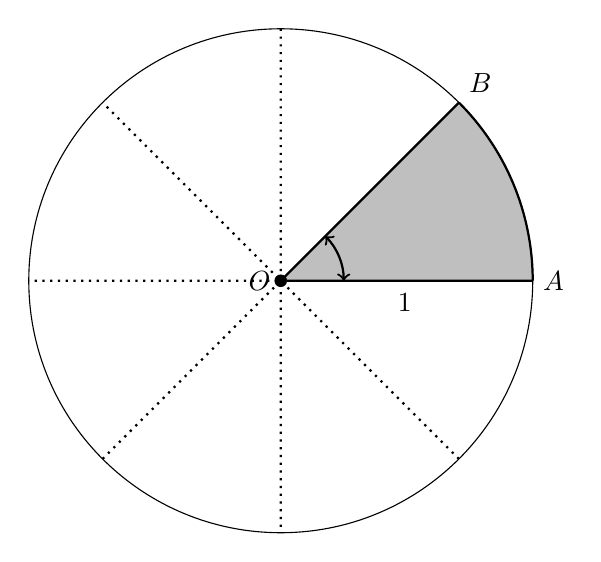
\begin{tikzpicture}[scale=0.8]
    \fill [lightgray]
    (0,0)--(0:4) arc (0:45:4)--(0,0);
    \draw (0,0) circle[radius=4];
    \draw [thick, <->] (0:1) arc (0:45:1);
    \draw [thick] (0:4) arc (0:45:4);
    \draw [thick]
    (0:4) node[right] {$A$}--
    (0,0) node[left] {$O$}--
    (45:4) node[above right] {$B$};
    \draw [thick, dotted](90:4)--(0,0)--(135:4);
    \draw [thick, dotted](225:4)--(0,0)--(180:4);
    \draw [thick, dotted](-45:4)--(0,0)--(-90:4);
    %\draw [thick, dotted](-135:4)--(0,0);
    \fill (0,0) circle[radius=.1];
    %\node at (18:4.5) {$?$};
    \node at (-10:2) {$1$};
  \end{tikzpicture}
  \end{multicols}

\newpage
\item Convert units of \emph{radians} and \emph{degrees} ($2 \pi = 360^\circ$, $\pi = 180^\circ$).\\[0.25cm]
  Apply the appropriate formula.
  \begin{multicols}{2}
    $\displaystyle d = r \times \frac{180}{\pi}$\\
    $\displaystyle r = d \times \frac{\pi}{180}$
  \end{multicols} \vspace{0.5cm}
  \begin{multicols}{2}
    \raggedcolumns
    \begin{enumerate}
      \item $\displaystyle m\angle A = \frac{\pi}{6}  =\hspace{0.15cm} ?$ degrees\\[0.75cm]
      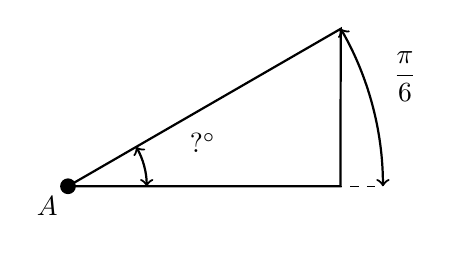
\begin{tikzpicture}[scale=1]
        \draw [thick, <->] (0:1) arc (0:30:1);
        \draw [thick, <->] (0:4) arc (0:30:4);
        \draw [dashed](0,0)--(4,0);
        \draw [thick]
        (0,0) node[below left] {$A$}--(30:4)--(3.46,0)--cycle;
        \fill (0,0) circle[radius=.1];
        \node at (18:1.8) {$?^\circ$};
        \node at (18:4.5) {$\displaystyle \frac{\pi}{6}$};
      \end{tikzpicture}
      \columnbreak
      \item $m\angle B = 45^\circ = \hspace{0.15cm} ?$ radians \\
      (in terms of $\pi$)\\[0.5cm]
      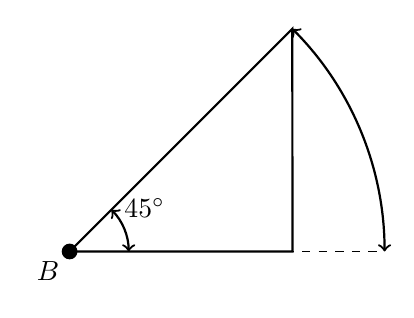
\begin{tikzpicture}[scale=1]
        \draw [thick, <->] (0:0.75) arc (0:45:0.75);
        \draw [thick, <->] (0:4) arc (0:45:4);
        \draw [dashed](0,0)--(4,0);
        \draw [thick]
        (0,0) node[below left] {$B$}--(45:4)--(2.83,0)--cycle;
        \fill (0,0) circle[radius=.1];
        \node at (30:1.1) {$45^\circ$};
      \end{tikzpicture}
    \end{enumerate}
  \end{multicols}

\newpage
\item Given a triangle $\triangle ABC$ having angles with measures $m\angle A = 37^\circ$ and $m\angle B = 78^\circ$. Find the measure of the third angle, $m\angle C$.
  
\newpage
\item The \emph{pie chart} below shows the proportion of two subsets of a population, one represented in blue and one in orange. Dotted lines divide the circle in six equal sectors for reference.
  \begin{multicols}{2}
  \raggedcolumns
  \begin{enumerate}[itemsep=1.5cm]
    \item Estimate the area of the blue sector as a fraction of the circle and as a decimal.
    \item The central angle of the orange sector measures $70^\circ$. Find the fraction of circle's area shaded orange as a fraction and a decimal.
  \end{enumerate}
  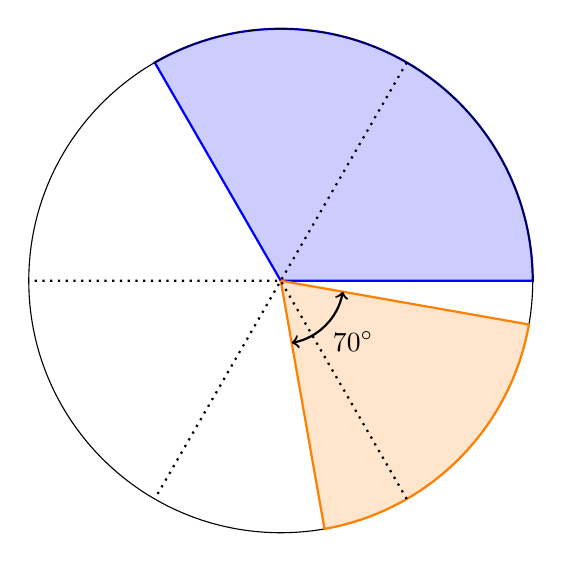
\begin{tikzpicture}[scale=0.8]
    \filldraw [color=blue, fill=blue!20, thick]
    (0,0)--(0:4) arc (0:120:4)--(0,0);
    \draw (0,0) circle[radius=4];
    \filldraw [color=orange, fill=orange!20, thick]
    (0,0)--(-10:4) arc (-10:-80:4)--(0,0);
    \draw [thick, <->] (-10:1) arc (-10:-80:1);
    \node at (-40:1.5) {$70^\circ$};
    \draw [thick, dotted](60:4)--(0,0)--(180:4);
    %\draw [thick, dotted](144:4)--(0,0)--(180:4);
    \draw [thick, dotted](-60:4)--(0,0)--(-120:4);
    %\draw [thick, dotted](0:4)--(0,0)--(-144:4);
  \end{tikzpicture}
  \end{multicols}

\newpage
\item Given circle with center $O$ and $m\angle QPR=31^\circ$. Find the measure of each arc or angle.
  \begin{multicols}{2}
    \raggedcolumns
    \begin{enumerate}[itemsep=1cm]
      \item $m \wideparen{QR}$
      \item $m\angle QOR$
      \item $m\angle POQ$
      \item $m\angle PQO$
    \end{enumerate}
      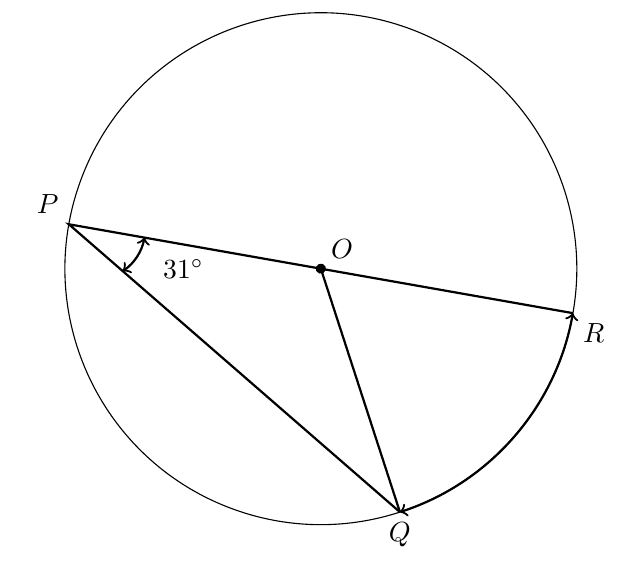
\begin{tikzpicture}[scale=.65, rotate=160]
        \draw (0,0) circle[radius=5];
        \fill (0,0) circle[radius=.1];
        \draw [thick]
        (190:5) node[below right] {$R$}--
        (0,0) node[above right] {$O$}--
        (128:5) node[below] {$Q$};
        \draw [thick] (0,0)--(10:5) node[above left] {$P$}--(128:5);
        \draw (20:2.1) node[left]{$31^\circ$};
        \draw [thick, <->] (128:5) arc (128:190:5);
        \draw [thick, <->] (10:3.5) arc (190:144:1);
      \end{tikzpicture}
  \end{multicols}

\newpage
\item The \emph{pie chart} below represents the population of the city of New York, with each borough's population a proportional sector.
  \begin{multicols}{2}
  \raggedcolumns
  Population of NY City is 8,336,000\\
  Population of the Bronx is 1,420,000
  \begin{enumerate}%[itemsep=1.5cm]
    \item Find the fraction of New Yorkers, $x$, who reside in the Bronx as a percentage. \vspace{2cm}
    \item Find the central angle of the shaded area, $\theta = x \times 360^\circ$
  \end{enumerate}
  \columnbreak
  \begin{flushright}
    New York City
  
  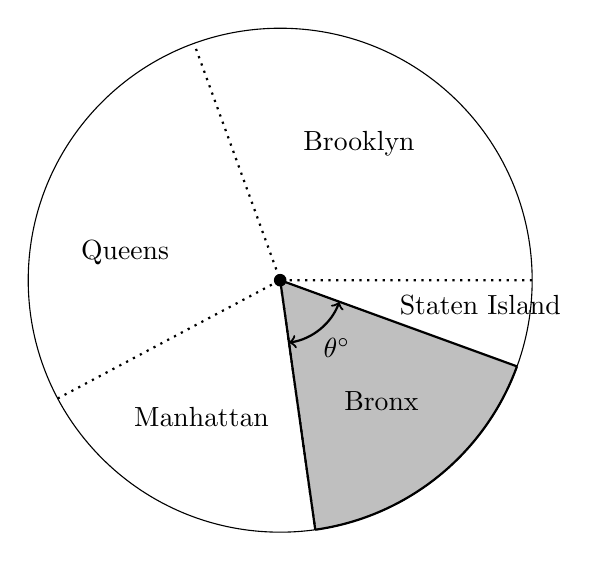
\begin{tikzpicture}[scale=0.8]
    \fill [lightgray] (0,0)--(-20:4) arc (-20:-82:4)--(0,0);
    \draw (0,0) circle[radius=4];
    \draw [thick, <->] (-20:1) arc (-20:-82:1);
    \draw [thick] (-20:4) arc (-20:-82:4);
    \draw [thick] (-20:4)--(0,0)--(-82:4);
    \draw [thick, dotted](208:4)--(0,0)--(278:4);
    \draw [thick, dotted](0:4)--(0,0)--(110:4);
    \fill (0,0) circle[radius=.1];
    \node at (-50:1.4) {$\theta^\circ$};
    \node at (60:2.5) {Brooklyn};
    \node at (170:2.5) {Queens};
    \node at (240:2.5) {Manhattan};
    \node at (-50:2.5) {Bronx};
    \node at (-7:3.2) {Staten Island};
  \end{tikzpicture}
  \end{flushright}
  \end{multicols}

\newpage
\item Right $\triangle ABC$ is drawn in \emph{standard position} with vertex $A$ on the origin and right $\angle C$ on the $x$-axis, as shown.
\begin{multicols}{2}
  \raggedcolumns
\begin{enumerate}
  \item Find the length of the hypotenuse $AB$ using the Pythagorean Theorem $a^2 + b^2 = c^2$. (leave as a radical)
  \vspace{3cm}
  \item Find the slope of the line segment $\overline{AB}$ as a decimal.
\end{enumerate}
  \begin{tikzpicture}[scale=0.7]
    %\draw [help lines] (-1.15,-1.2) grid (11,10);
    \draw [thick, ->] (-0.2,0) -- (9.4,0) node [above] {$x$};
    \foreach \x in {1,2,...,9}
      \draw[shift={(\x,0)},color=black] (0pt,2pt) -- (0pt,-2pt) node[below] {\footnotesize \; $\x$};
    \draw [thick, ->] (0,-0.2)--(0,9.6) node [left] {$y$};
    \foreach \y in {1,2,...,9}
      \draw[shift={(0,\y)},color=black] (-2pt,0pt) -- (2pt,0pt) node[left] {\footnotesize \; $\y$};
    \draw [-, thick] (0,0) node[below left] {$A$}
    --(8,0) node[above right] {$C$}
    --(8,4)node[right] {$B (8,4)$}--cycle;
    \draw (8,0)++ (-0.5,0)-- +(0,0.5)-- +(0.5,0.5);
    %\draw [<->, thick] (-0.6,4.3)--(5,8.5);
  \end{tikzpicture}
\end{multicols}
%https://graspablemath.com/canvas?load=_024bda2a5587c074

\newpage
\item Ten values from one to five are displayed as a dot plot below on the right. \\[0.5cm]
The data is to be represented as a \emph{pie chart}. The red sector has been drawn to represent data with value equalling five. (Dotted lines divide the circle in ten equal sectors for reference.)
  \begin{multicols}{2}
  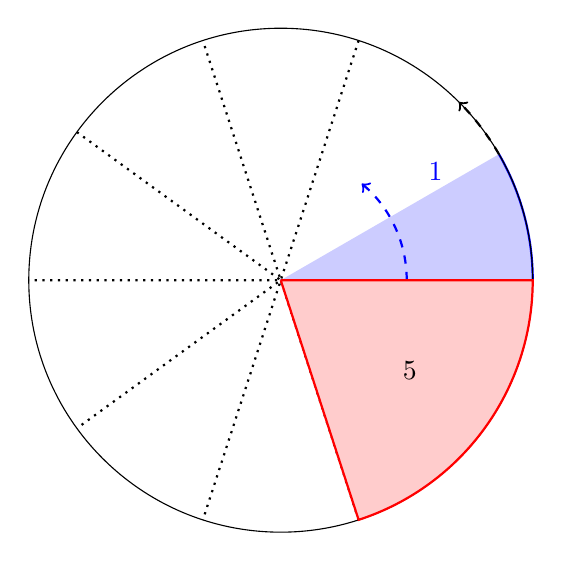
\begin{tikzpicture}[scale=0.8]
    \filldraw [color=blue, fill=blue!20, thick]
    (0,0)--(0:4) arc (0:30:4);
    \draw (0,0) circle[radius=4];
    \draw [thick, dashed, ->] (30:4) arc (30:45:4);
    \draw [color=blue, dashed, thick, ->] (0:2) arc (0:50:2);
    %\draw [thick]
    %(0:4) node[right] {$A$}--
    %(0,0) node[below left] {$O$}--
    %(36:4) node[right] {$B$};
    \draw [thick, dotted](72:4)--(0,0)--(108:4);
    \draw [thick, dotted](144:4)--(0,0)--(180:4);
    \draw [thick, dotted](-72:4)--(0,0)--(-108:4);
    \draw [thick, dotted](0:4)--(0,0)--(-144:4);
    \filldraw [color=red, fill=red!20, thick]
    (0,0)--(0:4) arc (0:-72:4)--(0,0);
    \node at (-35:2.5) {$5$};
    \node [color=blue] at (35:3) {$1$};
  \end{tikzpicture}
  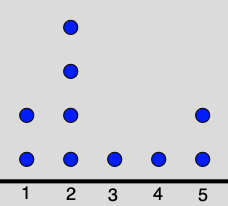
\includegraphics[width=5cm]{8-6_8DotPlot.png}
  \end{multicols}
  \begin{enumerate}
    \item Shade the appropriate portion of the pie chart in blue to represent the data with value equalling one.
    \item Complete the rest of the pie chart using other colors to mark sectors for the data equalling two, three, and four.
  \end{enumerate}

\newpage
\item Convert between units. \\[0.25cm]
General method: if $A = B$ multiply by $\displaystyle \frac{A}{B} \text{ or } \frac{B}{A}$. For example, $\pi \text{ radians}= 180 \text{ degrees}$ so \\
$\displaystyle r = d \times \frac{\pi}{180}$ and 
$\displaystyle d = r \times \frac{180}{\pi}$
\vspace{0.5cm}
  \begin{multicols}{2}
  \raggedcolumns
  \begin{enumerate}[itemsep=1.5cm]
    \item $35^\circ = \hspace{0.15cm} ?$ radians
    \item $\displaystyle \frac{\pi}{9}  = \hspace{0.15cm} ?$ degrees
    \item 1 foot = 12 inches\\[0.5cm]
    4.25 feet = 
    \item 70 inches = 
    \item 1 euro = 1.21 dollars\\[0.5cm]
    50 euro = 
    \item 50 dollars = 
    \item 1 mile = 5,280 feet\\[0.5cm]
    11,000 feet = 
    \item $\displaystyle \frac{3}{4}$ mile =   
  \end{enumerate}
  \end{multicols}
    
\newpage
\item Line segment $\overline{AB}$, $A(2,1)$, $B(10,7)$, is the diameter of circle $M$. 
\begin{enumerate}
  \item On the grid, mark and label as a coordinate pair the midpoint of the segment, the circle center $M$. 
  \item Calculate the length of $\overline{AB}$ and hence, the radius of the circle.\
  \item Write down the equation of the circle. 
  \item Sketch the circle on the grid or draw it with Geogebra or Graspable Math.
\end{enumerate}
\begin{flushright}
  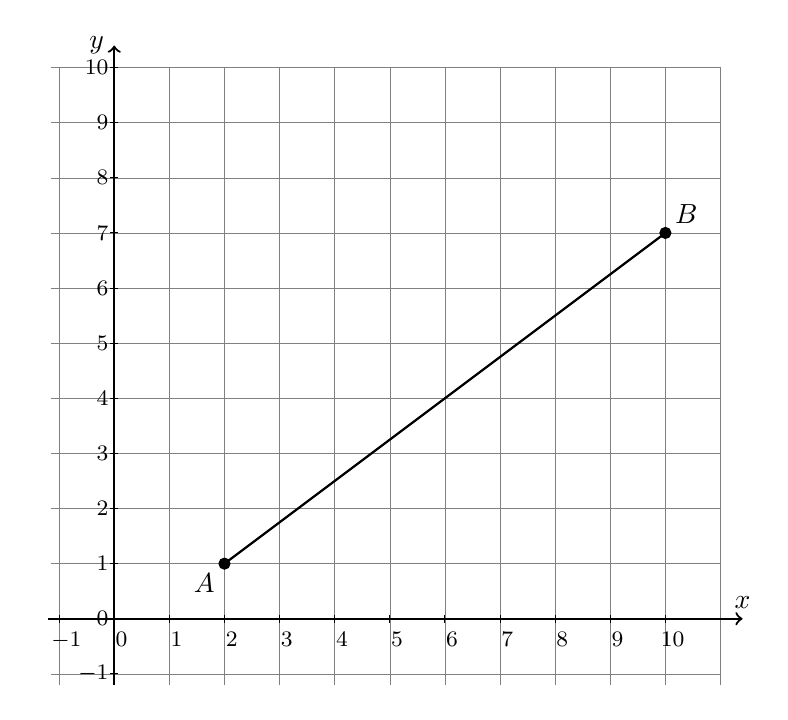
\begin{tikzpicture}[scale=0.7]
    \draw [help lines] (-1.15,-1.2) grid (11,10);
    \draw [thick, ->] (-1.2,0) -- (11.4,0) node [above] {$x$};
    \foreach \x in {-1,0,...,10}
      \draw[shift={(\x,0)},color=black] (0pt,2pt) -- (0pt,-2pt) node[below] {\footnotesize \; $\x$};
    \draw [thick, ->] (0,-1.2)--(0,10.4) node [left] {$y$};
    \foreach \y in {-1,0,1,...,9, 10}
      \draw[shift={(0,\y)},color=black] (-2pt,0pt) -- (2pt,0pt) node[left] {\footnotesize \; $\y$};
    %\draw [thick] (6,3) circle [radius=5];
    \draw [fill] (2,1) circle [radius=0.1] node[below left] {$A$};
    \draw [fill] (10,7) circle [radius=0.1] node[above right] {$B$};
    \draw [-, thick] (2,1)--(10,7);
    %\draw [<->, thick] (-0.6,4.3)--(5,8.5);
  \end{tikzpicture}
  \end{flushright}
  %https://graspablemath.com/canvas?load=_024bda2a5587c074
  %https://graspablemath.com/canvas?load=_6a89b545540e2be5


\end{enumerate}
\end{document}